\documentclass[12pt,headsepline]{scrartcl}

\usepackage{amsmath}
\usepackage{amsfonts}
\usepackage[utf8]{inputenc}
\usepackage[ngerman]{babel}
\usepackage[T1]{fontenc}
\usepackage[math]{blindtext}
\usepackage{scrpage2}
\usepackage{graphicx}
\usepackage{array}
\usepackage{longtable}
\usepackage{hyperref}

\cfoot{} \ifoot{} \ofoot{}\chead{}
\pagestyle{empty}
\begin{document}
\begin{center}

\includegraphics[]{icon_android.png}

\textbf{\Huge{Vertretungsplan-App}}

Informatik-Projekt am St. Michael Gymnasium Ahlen
\end{center}
\vspace{6cm}
\tableofcontents

\newpage
\setcounter{page}{1}
\pagestyle{headings}
\cfoot{} \ifoot{} \ofoot{}\chead{}
\ohead{\pagemark}
\ihead{\rightmark}
\pagestyle{scrheadings}

\section{Einführung}
Hey du.
Wie ich höre hast du vor die Vertretungsplan-App zu begleiten. Lass dir gesagt sein, dass dieses Projekt andere Qualitäten abverlangt als der ``normale'' Informatik-Unterricht es tut. Aufgrund dessen sind auch einige wenige Voraussetzungen zu erfüllen, da du sonst keinen Spaß hast dieses Projekt zu begleiten. Du musst Spaß am Programmieren haben, so hat es bei mir angefangen. Jedoch musste ich schnell feststellen, dass eine App zu schreiben nicht nur das Programmieren beinhaltet, denn die Plattform, also das Android-Betriebssystem, bringt einige Voraussetzungen, in die man sich einlesen muss. Auch Kreativität ist wünschenswert, denn gelegentlich darf man auch mal ein Bild erstellen oder sich generell das Layout der App überlegen. Die Hardware-technischen Voraussetzungen sind leider auch gegeben. Ein Android-Handy ist von großem Vorteil, aber nicht zwingend notwendig, da man dieses auch auf dem Computer simulieren kann. 
So kommen wir zum nächsten, Zugriff zu einem Computer ist unabdingbar und nicht die 
Schulrechner, auf denen man nichts installieren kann, sondern am Besten ein eigener zu Hause. Wo ich gerade von zu Hause spreche, dies ist sicherlich eine perfekte Gruppenarbeit, denn das Einarbeiten in die Android-Programmierung und eventuell auch in (meine) Vertretungsplan-App dürfte in einer Gruppe deutlich unterhaltsamer und eventuell auch schneller von Statten gehen, wenn man sich gegenseitig dabei hilft.

Was bringt einem dieses Projekt denn eigentlich, magst du dich fragen. Zum einen hilfst du deinen Mitschülern, welche die App benutzen, zum anderen wirst du einiges über die Android-Programmierung erfahren, aber auch in einem gewissen Maße, wie ein Android-Handy funktioniert. Auch wirst du erfahren, wie man solch ein Projekt mit Git organisiert.
\newline
\textbf{Nochmal: Gruppenarbeit ist sehr wünschenswert :)}
\newpage
\section{Aller Anfang ist mühsam}

Du möchtest dich jetzt erst mal langsam an Android antasten, was völlig verständlich ist. Dazu gibt es hier eine ausführliche Anleitung: \url{https://developer.android.com/training/basics/firstapp/index.html}. Als Programmierumgebung empfehle ich Android Studio, was seit 2015 die Standardumgebung für Android-Programmierung ist. In der Anleitung wird auch erklärt, wie man die Android SDK herunterlädt, außerdem wirst du beim Erstellen deiner ersten App begleitet. Bei Problemen einfach googlen oder auf \url{http://www.stackoverflow.com} suchen, welches eine sehr gute Hilfe ist.
Damit hast du dann schon deine erste Android-App programmiert. Auch wenn du jetzt etwas erschlagen bist, so hast du doch bis jetzt sehr viel erreicht. Wenn du hierfür etwas länger brauchst ist das völlig normal, ich hab auch erst einmal eine kleine simple App programmiert, um mich heranzutasten.

\section{Das Vertretungsplan-Projekt}
\subsection{Die Vorbereitungen}
Du solltest jetzt dein erstes Android-Programm auf einem Emulator, oder noch besser auch auf einem Android-Smartphone, ans Laufen gebracht haben. Nun gilt es das Vertretungsplan-Projekt in Android Studio zu laden und dieses zu starten.
Genutzt wird \href{http://git-scm.com/}{Git}, es verwaltet Versionen von Dateien, in unserem Fall von den Programmdateien unseres Projektes. Zum Speichern der Daten im Internet benutzen wir \href{http://www.github.com}{GitHub}. Um das Projekt herunterzuladen benötigst du keinen Account. Wenn du später die Änderungen und Verbesserungen, die du gemacht hast, wieder hochladen möchtest, musst du einen Account bei GitHub haben, welcher kostenlos ist. Ich empfehle dir also jetzt schon einen Account anzulegen und eventuell auch ein Testprojekt hochzuladen um die Features, die Git und GitHub bieten, auszuprobieren. Zu Git und GitHub gibt es hier eine sehr gute Anleitung: \url{https://help.github.com/}. Danach solltest du wissen, was z.B. ein Commit ist und auch, wie du deine Änderungen nach GitHub ``pusht''.
Mein Repository kannst du hier finden: \url{https://github.com/He-Ro/Vertretungsplan-App/}, die Webseite kannst du hier besuchen: \url{http://he-ro.github.com/Vertretungsplan-App}.
Um nun Lese- und Schreib-Rechte auf meine Repository zu erhalten benötigst du einen Key, den ich zunächst erstellen muss, wie es hier beschrieben ist \url{https://help.github.com/articles/generating-ssh-keys}, dort steht auch, wie du den öffentlichen Key importieren kannst.
Der Code kann in Android Studio direkt von GitHub heruntergeladen werden, gehe dazu aur \textit{VCS $\rightarrow$ Checkout from Version Control $\rightarrow$ Git}. Wenn du \textit{GitHub} benutzt musst du deinen GitHub Account mit Android Studio verknüpfen, was aber nicht notwendig sein sollte.
Lass das Projekt jetzt laufen; bei Problemen googlen :)
\newpage
\subsection{Der Aufbau des Projektes}
Den Aufbau eines Android Programms solltest du jetzt kennen, nämlich, dass im \textit{src}-Ordner die Java-Dateien liegen. Im \textit{res}-Ordner die Ressourcen, also vor allem die Layout-XLM-Dateien, die Bild-Dateien, die statischen Strings, und so weiter. Und dass die \textit{AndroidManifest.xml}-Datei einfach im Projektordner liegt.
Zunächst einen Überblick über das Programm und die Klassen, die dazugehören:
\begin{center}
\begin{longtable}{p{5cm}p{5cm}p{5cm}}
\textbf{Hauptscreen} & \textbf{Optionen} & \textbf{Widget}\\
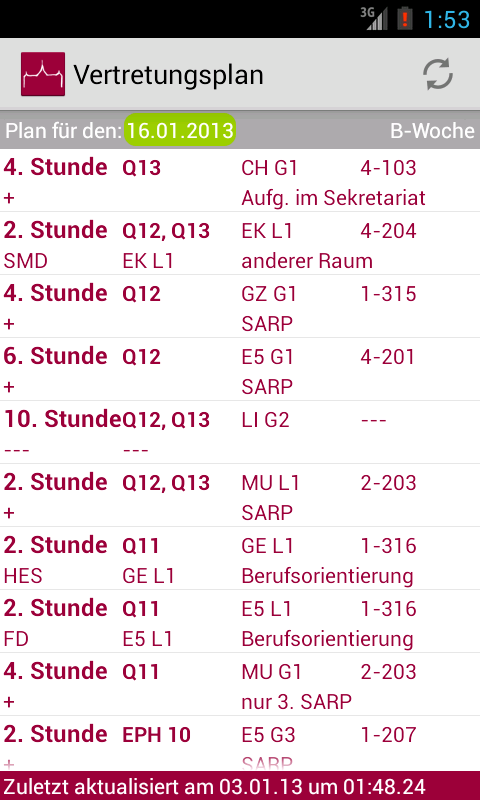
\includegraphics[scale=0.28,keepaspectratio=true]{device-2013-01-16-103322.png}
&
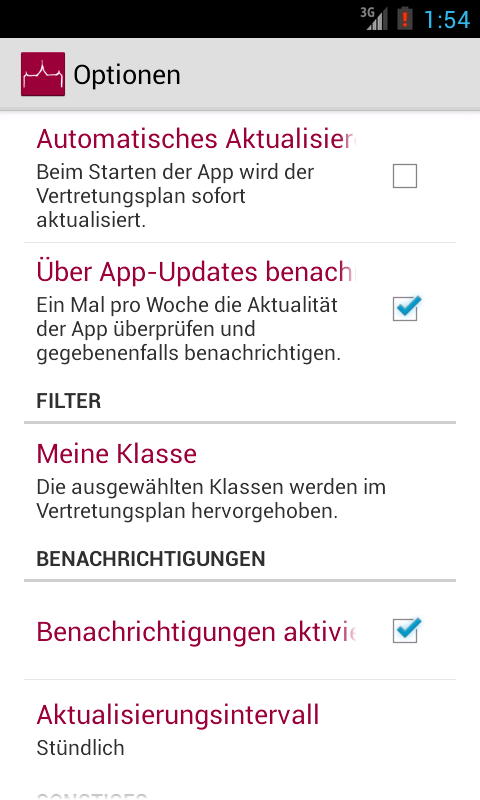
\includegraphics[scale=0.28,keepaspectratio=true]{device-2013-01-16-103407.png}
&
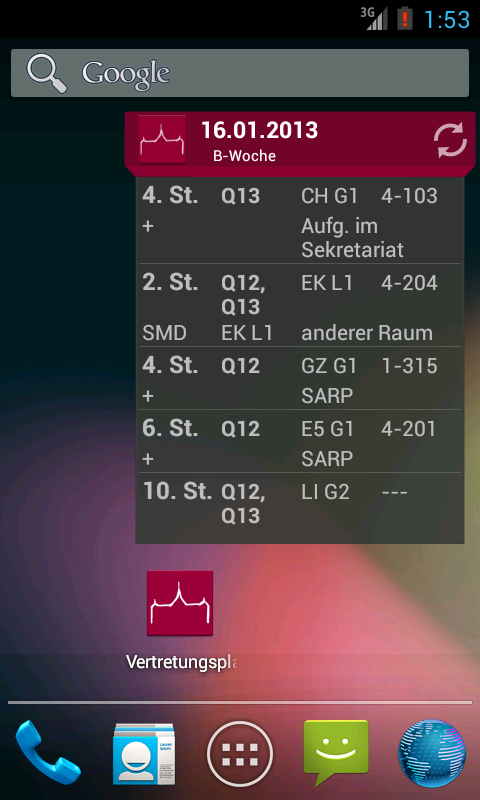
\includegraphics[scale=0.28,keepaspectratio=true]{device-2013-01-16-103244.png}\\
Diese Liste zeigt den Vertretungsplan an. &
In den Optionen kann der Benutzer die Einstellungen ändern. &
Das Widget zeigt den Vertretungsplan auf dem Homescreen an.\\
\underline{Die dazugehören Java Klassen:}& & \\
\begin{itemize}
 \item MainActivity
 \item MyListAdapter
\end{itemize} &
\begin{itemize}
 \item PrefsActivity
\end{itemize} &
\begin{itemize}
 \item WidgetProvider
 \item WidgetService
 \item WidgetUpdate
 \item WidgetViewsFactory
\end{itemize}\\
\newpage
\underline{Dazugehörige wichtige Ressourcen:}& & \\
\begin{itemize}
 \item layout/main.xml
 \item layout/costum \_row\_view.xml
 \item menu/menu.xml
\end{itemize} &
\begin{itemize}
 \item xml/preferences.xml
 \item layout/ueber\_dialog \_layout.xml
\end{itemize} &
\begin{itemize}
 \item xml/widget\_ provider.xml
 \item layout/widget.xml
 \item layout/costum \_row\_view.xml
\end{itemize} \\
\end{longtable}

\end{center}
\underline{Klassen, die im Hintergrund laufen}\\
\small{Und deshalb nicht zu einer der drei Screens gehören.}
\begin{itemize}
 \item CheckForAppUpdate
 \item CheckForUpdates
 \item HtmlWork
 \item OnBoot
\end{itemize}
Detaillierte Informationen zu den einzelnen Klassen und Ressourcen sind als Kommentare in den einzelnen Dateien zu finden. 
\subsection{Eine neue Version veröffentlichen}

Wir nehmen jetzt an, dass du ein paar Änderungen an der App vorgenommen hast und bist der Meinung, dass die neue Version stabiler/besser läuft als die Alte.
Um diese Version zu veröffentlichen sind einige Maßnahmen zu treffen, diese liste ich hier auf:
\begin{enumerate}
 \item Setzte den \texttt{android:versionCode} in dem \textit{AndroidManifest} um genau einen hoch. Merke dir diese neue Versionsnummer.
 \item Gib der Version einen sinnvollen Namen, dies hat nichts mit dem \texttt{android:versionCode} zu tun und ist in \textit{res/values/strings.xml} zu finden unter \texttt{version\_nr}. Wenn die aktuelle Version z.B 0.3.2 ist und du nur kleine Bug-Fixes veröffentlichst, solltest du die letzte Nummer um Eins erhöhen, sodass es 0.3.3 wird. Bei neuen Funktionen kannst du die zweite Nummer um Eins erhöhen und die letzte auf Null setzen, also 0.4.0. Bei einer GANZ neuen Funktion, z.B. das Laufband ist mit hinzugefügt, das Layout wurde grundlegend verändert o.ä. kannst du die erste Zahl um Eins erhöhen, dass es 1.0.0 wird. (Infos: \href{https://de.wikipedia.org/wiki/Version_\%28Software\%29}{\texttt{https://de.wikipedia.org/wiki/Version\_(Software)}})
 \item Nun exportierst du die apk-Datei, dies ist in Android Studio sehr einfach. Gehe dazu auf \textit{Build $\rightarrow$ Generate Signed APK\dots}. Die keystore-Datei ist in dem Projektordner gespeichert, das Passwort dazu musst du dir von Frau Terveer holen. Weitere Infos zum Signieren gibt es hier: \url{https://developer.android.com/tools/publishing/app-signing.html}. 
 \item Diese apk-Datei kann nun auf dem Android-Handys installiert werden. Dies solltest du am Besten noch einmal testen. Benenne die Datei so um, dass der Dateiname den Versionsnamen aus 2. enthält, also z.B. \texttt{Vertretungsplan\_0.3.apk}.
 \item Die apk-Datei muss nun hoch geladen werden, damit deine Mitschüler Zugriff auf die neue Version haben. Kopiere die apk-Datei dazu in den Ordner \texttt{Veroeffentlicht} und füge die Datei zu deinem Git-Repository hinzu. Nun änderst du die Versionsnummer in der Text-Datei \texttt{vertretungsplan\_version.txt} zu der Nummer von 1.  Dies bewirkt, dass die Klasse \texttt{CheckForAppUpdate} beim nächsten Check weiß, dass es eine neue Version gibt. Diese Änderungen werden nun ``comitted'' und zu GitHub ``gepusht''.
 \item Nun muss nur noch der Link auf der Webseite abgeändert werden. Der Link befindet sich natürlich in der index.html-Seite der Webseite, welche ein eigener Zweit(Branch) in GitHub ist. Diesen kannst du ``auschecken'' und dann lokal auf deinem Rechner bearbeiten, oder, weil es nur eine kleine Änderung ist auch in GitHub online. Den Link kannst du folgendermaßen erhalten. Gehe in GitHub im Zweig \texttt{master} auf \texttt{Veroeffentlicht}, dann auf die neue Version. Hier machst du einen Rechtsklick auf \text{Raw} und kopierst die URL-Adresse. Dies ist dann der Direktlink auf die neue Version, welche du in \texttt{index.html} einfügst.
 \end{enumerate}
 Glückwunsch!! Du hast jetzt eine neue Version veröffentlicht. Wenn deine Mitschüler die Option zum Überprüfen der Aktualität, dürften diese innerhalb der nächsten Woche eine Meldung erhalten.

\section{Das Projekt weitergeben}
Wenn du dann schließlich auch das Abitur schaffst und von der Schule gehst musst du natürlich das Projekt so vorbereiten, dass es auch an jüngere Mitschüler weitergegeben werden kann. Hierzu solltest du diese Datei(\LaTeX-Datei) anpassen, sodass es den jetzigen Stand widerspiegelt, hierzu gehört auch das Eintragen in die Autorenliste, sowie in der App um ``Über''-Menü. Außerdem solltest du das Programm gut kommentieren, so wie man es immer macht!!

\section{Mitwirkende}
\subsection{Schüler}
\begin{itemize}
 \item Hendrik Rosendahl (2012/13) \href{mailto:vertretungsplanapp-hero@yahoo.de?subject=Vertretungsplan-App}{\texttt{vertretungsplanapp-hero@yahoo.de}}
\end{itemize}
\subsection{Lehrer}
\begin{itemize}
 \item Frau Terveer (2012 - ...)
\end{itemize}


\end{document}
